\chapter{MacroLab} 
\label{sect:approach}

MacroLab allows the user to write a single program that is
simple, robust, and manageable and then automatically decomposes it
depending on the target deployment.  A {\em program decomposition} is
a specification of where data is stored in the network and how
messages are passed and computations are performed in order to execute
the program.  A macroprogram may be decomposed into {\em
  distributed} operations for a large mesh network, where data is
stored on every node and network operations are performed in-network.
It could also be decomposed into {\em centralized} operations for a
small star topology, where all data is collected to a central base
station.  A program may also be decomposed into many points on the
spectrum between purely centralized or purely distributed code. 
The implementation could also use group-based data processing
or in-network aggregation.

%% \begin{figure}
%%   \centering
%%   \includegraphics[width=1\columnwidth]{../fig/Macroprogram.eps}
%%   \smallskip
%%   \hrule
%%   \caption{MacroLab will compile a program into one of several alternative
%%     implementations, depending on the target deployment scenario.}
%%   \label{fig:dscd}
%% \end{figure}

\begin{figure}[h]
  \centering
  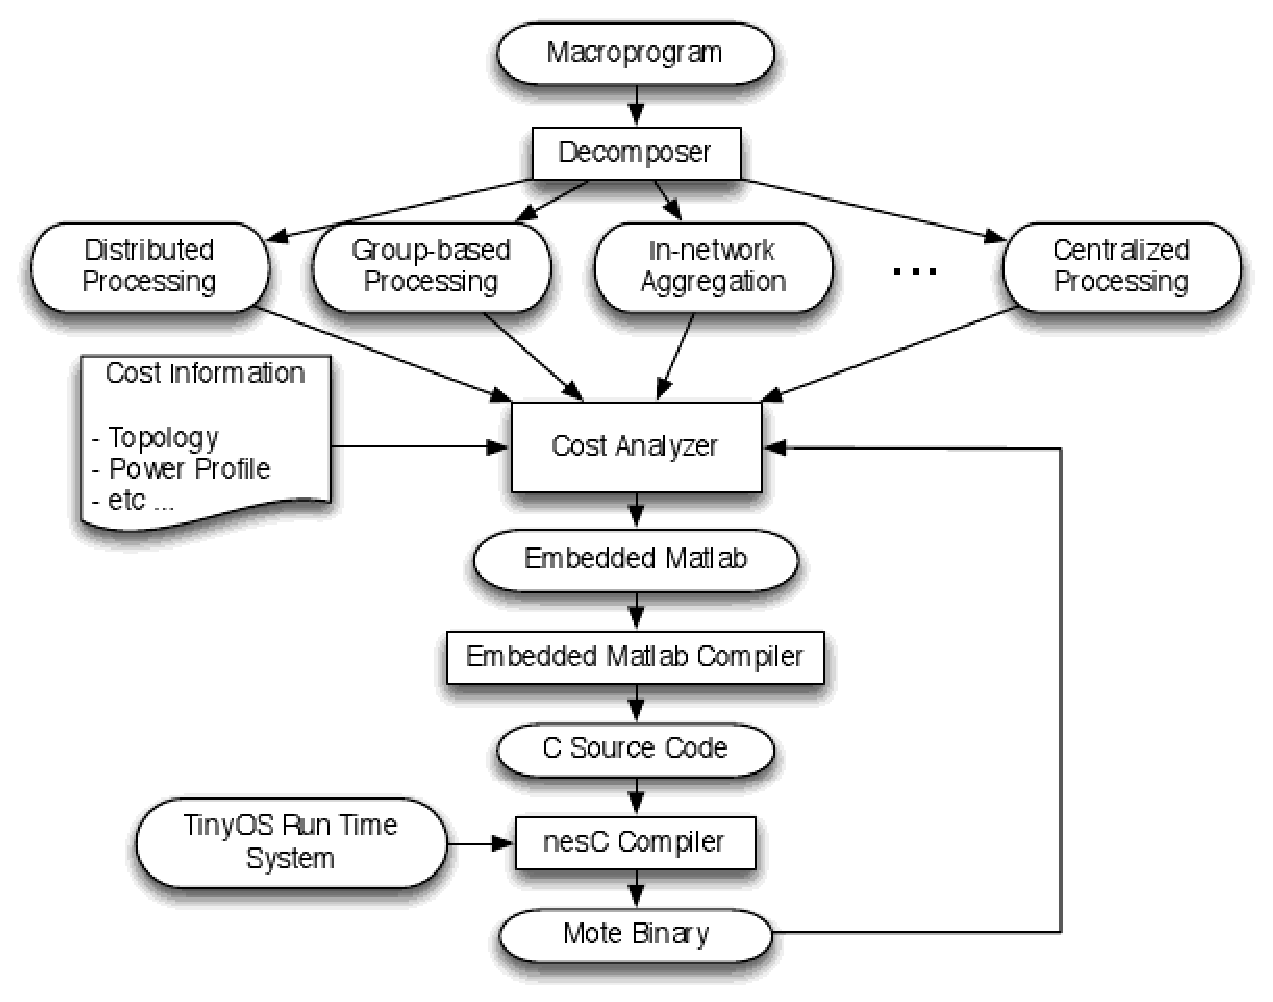
\includegraphics[width=0.8\columnwidth]{fig/System.eps}
  \caption[MacroLab system architecture]{MacroLab consists of a decomposer, a
  cost analyzer, and a run-time system. In our implementation, we generate all
  possible decompositions of a macroprogram and then analyze and compare them
  based on the cost profile of a target deployment.}
  \label{fig:System}
\end{figure}

MacroLab's overall architecture is depicted in Figure~\ref{fig:System}. 
A macroprogram (described in Section \ref{sect:abstraction}) 
is passed to the decomposer (Section \ref{sect:decomposer}) which 
generates multiple decompositions of the macroprogram.
Each decomposition is passed to the cost analyzer (Section
\ref{sect:costAnalyzer}) which calculates the cost of each with respect to
the cost profile of the target deployment. This cost profile must be
provided by the user and may include information such as the topology,
power restrictions, and descriptions of the radio hardware. The cost
analyzer chooses the best decomposition and passes it to the compiler and run-time
system (Section \ref{sect:RTS}) which converts the decomposition into a binary
executable and executes it.  While it executes,
the program and the run-time system continue to collect information about
the cost profile of the deployment and feed this information back to the
cost analyzer.  If the cost profile changes or if the cost profile at
compile time was incomplete or incorrect, the cost analyzer may decide to
reprogram the network with a new decomposition.

\begin{figure}
  \centering
  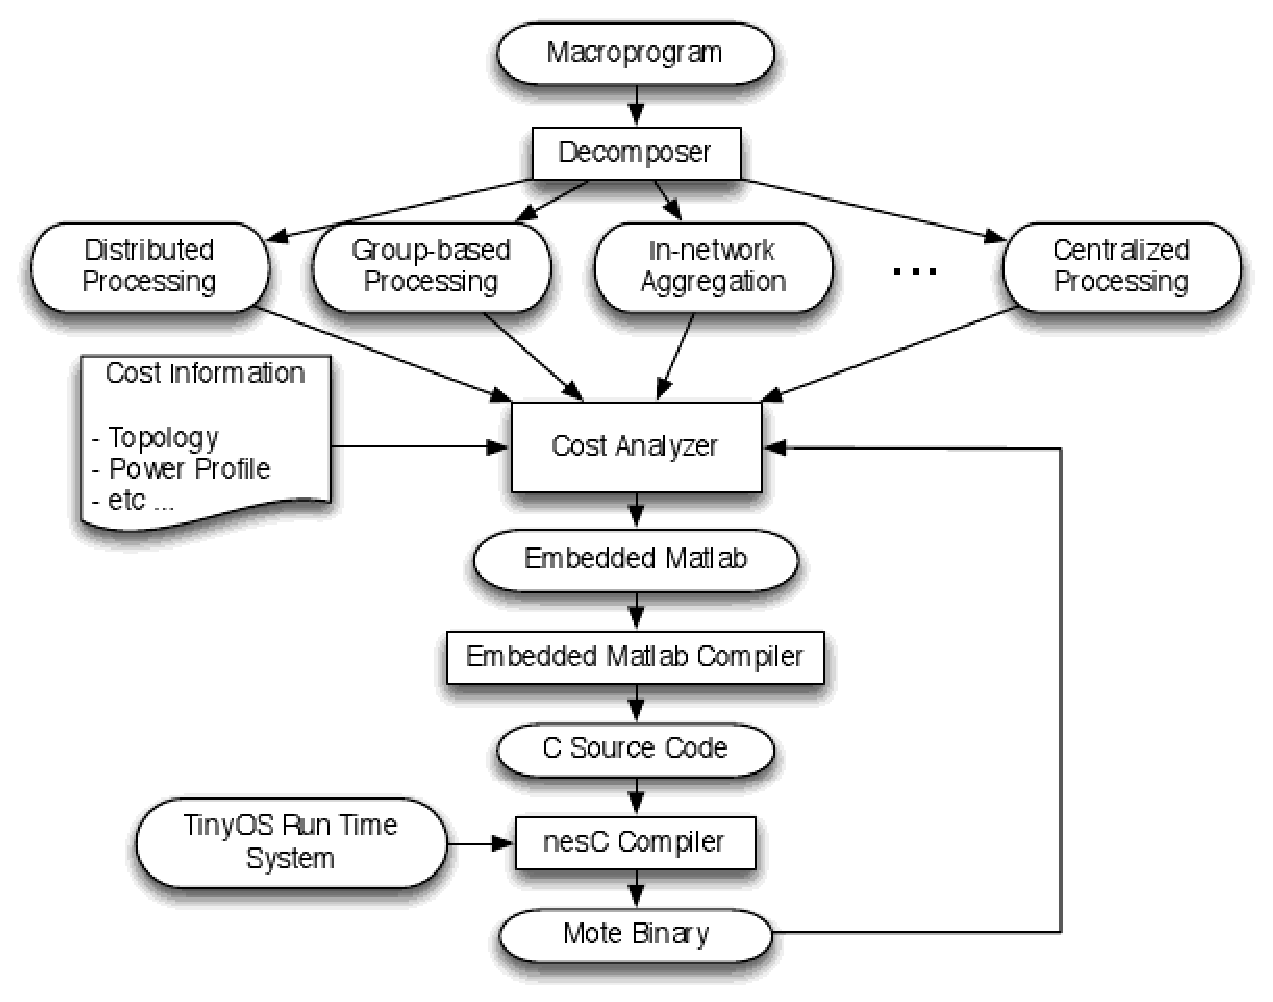
\includegraphics[width=1\columnwidth]{fig/System.eps}
  \smallskip
  \hrule
  \caption[MacroLab system architecture]{MacroLab consists of a decomposer, a cost analyzer, and a run-time
    system. In our implementation, we generate all possible decompositions of a
    macroprogram and then analyze and compare them based on the cost profile of
    a target deployment.}
  \label{fig:System}
\end{figure}

%% %% % An alternative implementation we considered is presented in Figure~\ref{fig:Alternative}, were the compiler uses the cost
%% %% % profile information to produce the correct decomposition the first time.  This
%% %% % is a simpler architecture, but in practice we found that it
%% %% % added unnecessary complexity to the compiler, and that it is easier to evaluate
%% %% % a decomposition given a cost profile than to produce one.

The architecture of MacroLab is presented in~\ref{fig:System}. An alternative
implementation would be a compiler using the cost profile implementation to
produce the correct decomposition the first time, but it is conceptually easier
to enumerate all possible implementations and evaluate them. 

In the following subsections, we discuss the four components of MacroLab: the
programming abstraction, the decomposer, the cost analyzer, and the run-time
system.

\section{Abstraction} \label{sect:abstraction}

MacroLab provides a {\em vector programming} abstraction similar to Matlab. A
vector is a data structure containing values called {\em elements}
that are arranged in rows and columns.  For example,
\[ r = \left[ \begin{array}{ccc}
a & b & c \\ d & e & f \\ g & h & i \end{array} \right]\] is a 3 x 3 vector with
9 elements.  Vectors can be indexed by dimension: the element in the second row
and the third column of $r$ can be selected with {\tt r(2,3)} resulting in $f$.
In MacroLab, like in Matlab, the ``{\tt :}'' is used to select an entire
dimension.  For example, {\tt r(3,:)} selects the 3rd element of the first
dimension (rows) and the entire second dimension (columns), namely {\tt
  [g~h~i]}.  Operations such as {\em vector addition} and {\em vector
  multiplication} operate on the data structures. The operation {\tt find(r==f)}
produces the index of the element in $r$ that has the value $f$, which is
$[2,3]$.  In addition to standard vector programming, MacroLab introduces three
new concepts to facilitate software development for CPSs: the macrovector, the
dot-product index, and the neighborhood.  These concepts are discussed in the
next three subsections.


\subsection{The Macrovector}

In MacroLab, we define a new data structure called the {\em macrovector}.
Macrovectors differ from traditional vectors in that each element of a
macrovector is associated with a particular node in the network.
Thus, macrovectors are \emph{unordered} and are \emph{indexed by node ID}.
This abstraction can be useful, for example, to store sensor readings. If
{\tt light} is a macrovector storing the light values of each sensor,
then the operation {\tt light(5)} would retrieve the light value of the sensor
node with $ID=5$. Since sensor node IDs may be non-sequential, the elements
in a macrovector do not form a strict sequence.
Macrovectors can have multiple dimensions, but only a single dimension is
indexed by node ID.  The other dimensions are normal vectors indexed sequentially.
Macrovectors can be created using the command
\vspace{.1in}
\begin{center}
\ttfamily\small
\begin{verbatim}
light = Macrovector(<scope>, [length], [length], ...)
\end{verbatim}
\end{center}
\vspace{.1in} 
\noindent where the {\tt scope} of the macrovector is the set of nodes
with which the elements are associated.  This scope is a vector of node
IDs and the length of the first dimension will be the number of IDs.  The
lengths of subsequent dimensions must be given for a multi-dimensional
macrovector. These {\tt length}s are simply integer values indicating the
size of each dimension.

Macrovectors support many standard Matlab vector operations such as {\tt
addition}, {\tt subtraction}, {\tt cross-product}, {\tt find}, {\tt max}, and
{\tt min}.  These operations can be combined to perform {\em macro}
operations that operate on data associated with many different sensor
nodes.  For example, the operation
\vspace{.1in}
\begin{center}
\ttfamily\small
\begin{verbatim}
maxLight = max( light )
\end{verbatim}
\end{center}
\vspace{.1in}
will return the maximum light value in the network.  
The operation
\vspace{.1in}
\begin{center}
\ttfamily\small
\begin{verbatim}
brightNodes = find( light > mean(light))
\end{verbatim}
\end{center}
\vspace{.1in}
will return the IDs of nodes that have above-average light values.  
The operation
\vspace{.1in}
\begin{center}
\ttfamily\small
\begin{verbatim}
hotLight = light( find( temp > 100 ) )
\end{verbatim}
\end{center}
\vspace{.1in}
will return the light values on nodes where the {\tt temp} value is higher
than 100.  If these vectors were tables in TinyDB, this would be similar
to posing the SQL query
\vspace{.1in}
\begin{center}
\ttfamily\small
\begin{verbatim}
SELECT light WHERE temp > 100
\end{verbatim}
\end{center}
\vspace{.1in}

\begin{figure}
  \centering
  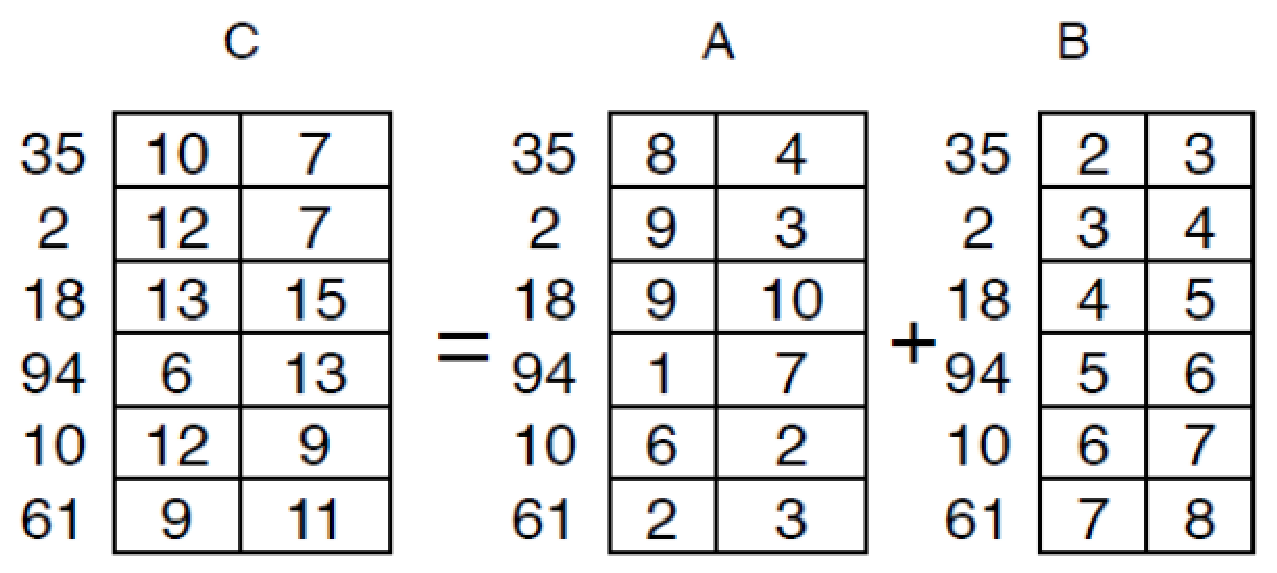
\includegraphics[width=1\columnwidth]{fig/DistributedArray1.eps}
  \smallskip
  \hrule
  \caption[Example of a distributed macrovector]{Two $n \times 2$ macrovectors $A$ and $B$ can be added and stored
    into a third macrovector $C$. The values on the left of each vector indicate
    which node ID the cells are associated with.}
  \label{fig:macroVectorAddition}
\end{figure}

Elements associated with the same node ID are paired together for binary
operations that involve multiple macrovectors.  For example,
Figure~\ref{fig:macroVectorAddition} shows the operation {\tt C = A + B}
performed on three $n \times 2$ macrovectors. In this operation, the elements of
$A$ and $B$ corresponding to node $35$, for example, are added together and
stored in the elements of $C$ corresponding to node $35$.

\subsection{Dot-product Index} \label{sect:dotProduct}
We provide a new way of indexing into macrovectors called the {\em
dot-product index}.  For example, with {\tt s~=~[1~2~3]} and {\tt
  t~=~[2~1~3]}, the aforementioned vector {\tt r} can be indexed as follows:
 \[ r(s,t)[1,2] == \left[ \begin{array}{ccc}
  & b &   \\
d &   &   \\
  &   & i \end{array} \right]\]

The two values in square brackets indicate that the elements of the
first and second dimension indices should be matched pair-wise before
values are selected from the matrix.  Since $s$ and $t$ each contain 3
elements, this dot-product index would select 3 elements from $r$ in
total.  With the values of $s$ and $t$ above, the dot-product index
would select elements $[1, 2]$, $[2, 1]$, and $[3, 3]$.  This is
different from traditional indexing in Matlab, what we might call
the {\em cross-product index}, in which the same index vectors would
produce
\[ r(s,t) = \left[ \begin{array}{ccc}
b & a & c \\
e & d & f \\
h & g & i \end{array} \right]\]

\begin{figure}[t]
  \centering
  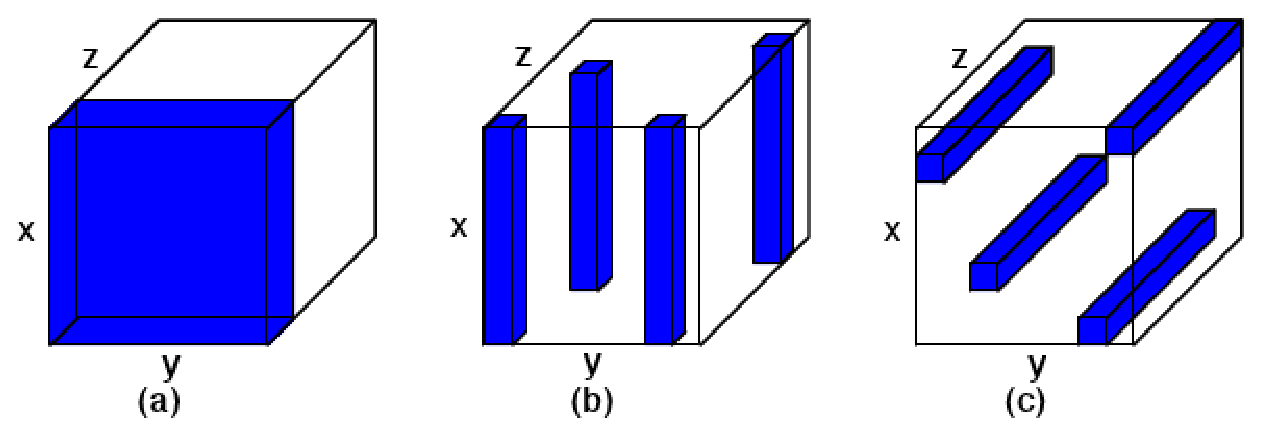
\includegraphics[width=1\columnwidth]{fig/DotProducts}
  \smallskip
  \hrule
  \caption[Example of dot-product indexing]{A three-dimensional vector $D$ can
    be indexed with the (a) cross-product index {\tt D(x,y,1)}; (b) dot-product
    index {\tt D(:,y,z)[2,3]}; or (c) dot-product index {\tt D(x,y,:)[1,2]}.}
  \label{fig:dotProduct}
\end{figure}

In other words, all values of index vector $s$ are paired with all values of
index vector $t$, selecting 9 values in total.  Figure~\ref{fig:dotProduct}
illustrates how cross-products and dot-products can be used to select
different elements in a three-dimensional vector.

Dot-product indexing can be used to efficiently perform operations in
which the element to be selected on each node is different.  For
example, if an $n \times 10$ macrovector {\tt circularBuffer} stored
the last 10 light values read on each node and an $n \times 1$
macrovector {\tt lastIndex} stored the index of the most recent value
stored, then the operation {\tt circularBuffer(:,lastIndex)[1,2]}
would provide the most recent value on each node. The capabilities of
macrovectors and dot-product indexing will be demonstrated
in Section~\ref{sect:evaluation}.

\subsection{Neighbor-based Representation} \label{sect:neighborRepresentation}
A node's {\em neighborhood} is the set of nodes that are within radio
range.  This is a very useful type of {\em group} in which a node is
guaranteed to have cheap communication to all other nodes. Connectivity-based neighborhoods are often
a critical part of efficient in-network data processing algorithms.
Neighborhoods are a special type of group since each node has a
different neighborhood.
Because of this, we introduce new syntax for defining a
neighbor-based macrovector:
\vspace{.1in}
\begin{center}
\ttfamily\small
\begin{verbatim}
lightReflection = neighborReflection(light)
\end{verbatim}
\end{center}
\vspace{.1in} 
\noindent which indicates that lightReflection is a vector of
neighbor-based macrovectors that should store {\em reflections} 
of the {\tt light} macrovector. When a node writes to its own element
of the {\tt light} macrovector, that value is cached in the rows
corresponding to its neighbors.  Thus, {\tt lightReflection} is a two
dimensional vector where each row contains cached values of a node's
neighbors' light readings. Since each node may have a neighborhood of
different size, this is not necessarily a rectangular matrix; each row may
be a different length.  This abstraction is very similar to the Hood
programming abstraction~\cite{Whitehousea}.

\subsection{Program Decomposition} \label{sect:decomposer}

%% %%\XXX{the intro to the compiler needs to really state the overall
%% %%  algorithm. Maybe a flow chart diagram would be nice.}

%% %% \XXX{what we previously called the ``compiler'' is now called the ``decomposer'' because it goes from macrocode to microcode.  We should describe the compilation process to be the process of going from microcode to executable.  I've already changed most of this text to replace ``compiler'' with ``system'' until we come up with a better name}.

The MacroLab decomposer converts a macroprogram into a set of
microprograms that can be executed on nodes.  The goal is to preserve
the semantics of the macroprogram while allowing for efficient
distributed operation.  The decomposition algorithm has two
steps. First, it chooses a data {\em representation} for each
macrovector, which can be {\em distributed}, {\em centralized}, or
{\em reflected} (Section~\ref{sect:decompositionTypes}).  Based on the
representations chosen, it then uses rule-based translation to convert
the vector operations in the macroprogram into network operations (Section~\ref{sect:codeTranslation}).

%% % Pieter - rewrite starts 

\subsection{Choosing Macrovector Representations}\label{sect:decompositionTypes}

\begin{figure}[t]
  \centering
  \subfigure[Distributed Macrovector: Nodes can read and write their own
  values in the vector.]{
  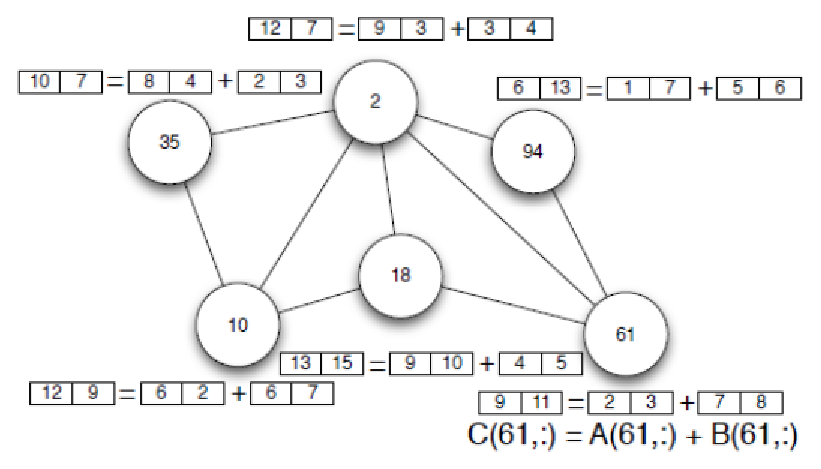
\includegraphics[width=0.6\columnwidth]{fig/DistributedArray.eps}
  \label{fig:distributedVector}
  } \subfigure[Reflected Macrovector: Nodes can read all values in the vector,
  but can only write to their own value.]{
  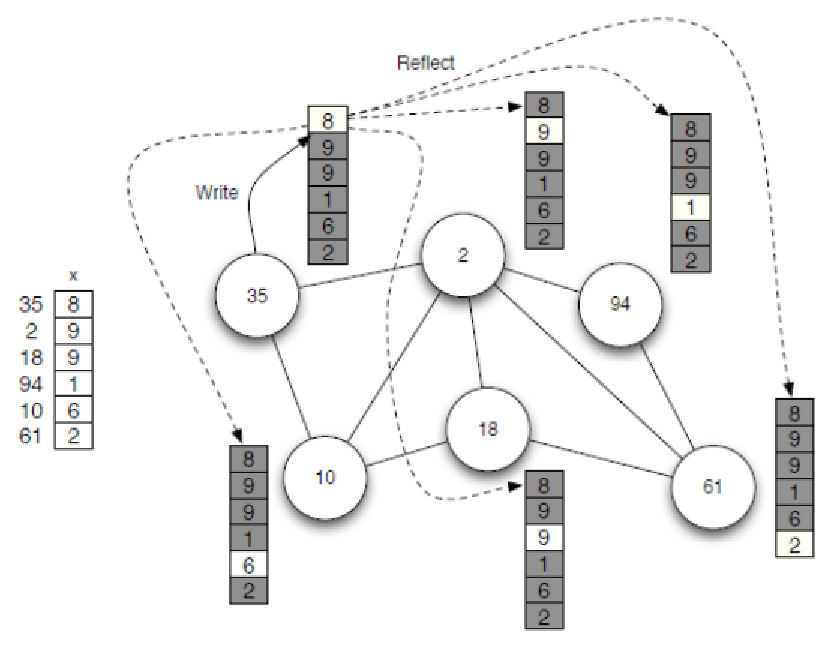
\includegraphics[width=0.6\columnwidth]{fig/ReflectedArray}
  \label{fig:reflectedVector}
  }
  \smallskip
  \hrule
  \caption[Example macrovector representations.]{Macrovectors can be
    (a) distributed across nodes or (b) reflected across nodes. They
    can also be represented in other ways that are not shown.}
\end{figure}

Macrovectors provide a uniform interface to several underlying {\em
  representations}, which are different ways that the macrovector can
be stored in the network.  MacroLab currently supports three
representations: distributed, centralized, and reflected, the
trade-offs of which are described in more detail below.  Other
representations are possible and would allow MacroLab to support
different classes of distributed algorithms.  Vector operations can be
applied to macrovectors regardless of their representation, making
them ideally suited for DSCD.

With three possible macrovector representations, a program with four
macrovectors would have $3^4$ possible decompositions.  Thus, the space of
decompositions grows exponentially with the number of macrovectors in a program.
Currently, MacroLab must systematically explore all possible combinations of
representations for the macrovectors in a program in order to find the optimal
decomposition.  This is currently not a problem for programs with only a small
number of macrovectors. For the programs described in this paper, the
translation process from macrocode to microcode takes less than 0.5 seconds.  In
contrast, compilation of the microcode to a binary executable takes over 13
seconds, using the nesC and Matlab compilers.

{\bf Distributed Representation:} The first way to represent a macrovector is to
store each row on its associated node.  Figure~\ref{fig:distributedVector} shows
how the elements of the macrovectors $A$, $B$, and $C$ from
Figure~\ref{fig:macroVectorAddition} can be stored on each node and how the {\tt
  addition} operation is performed. Since elements are only added to
corresponding elements on the same node, this operation can take place without
message passing between nodes.

In general, the distributed representation of macrovectors allows for the
efficient implementation of vector operations that do not span multiple rows.
Conversely, this representation requires significant message passing for
aggregate operations like {\tt max} that require values resident on multiple
nodes. If a macroprogram uses the {\tt max} operation frequently on a particular
macrovector, then a distributed decomposition would be very costly.

{\bf Centralized Representation:} The second representation supported
by our framework stores all elements on a single node, typically the
base station. This representation is in diametric opposition to a
\emph{distributed} representation. It allows operations like {\tt max}
to be applied with virtually no explicit message passing cost.
However, there is a potentially significant cost associated with keeping
the elements of the centralized vector up-to-date. If the values are
frequently updated remotely by the sensor nodes, they need to be
frequently transmitted for storage. The centralized
representation is favorable if the vector participates frequently in
aggregate operations that span rows (like {\tt max}). It is less
favorable if the vector is frequently updated with
sensor data.

{\bf Reflected Representation:} The third macrovector representation stores all
elements on all nodes. The microcode on each node has read/write access to its
associated element and read-only access to cached versions of all other elements
in the vector. This precludes the need for write-write synchronization since
only one node may write to any given element. However, nodes do need to
communicate their updated values after performing a write, as illustrated in
Figure~\ref{fig:reflectedVector}; when node $35$ writes to its own element in
the vector, the value is {\em reflected} to all other nodes currently caching
it.

This representation is conceptually similar to Reflective Memory (RM), which is
a form of shared memory for parallel systems\cite{Jovanovic}.  It is different
from a neighbor-based macrovector because the scope of a reflected macrovector
is {\em globally defined}; it is not different for each node.  The reflected
representation is beneficial when used by a small {\em group} of nodes that are
relatively close to each other but comparatively far from the base station. In
that situation, the cost of sending information to the base station to perform a
{\tt max} operation is higher than the cost of transmitting to all other nodes
in the group. The reflected representation may also make an operation cheaper
when all nodes need the result.

%% %% % Pieter - rewrite ends

%% %% % Pieter - commenting following subsection for now -- will break
%% %% % references elsewhere for the time being

%% %% %% \subsubsection{Applying Operators to a Decomposition}\label{sect:functionLibrary}

%% %% %%  %% \XXX{this section needs an intro paragraph that clearly
%% %% %% enumerates all of the parts.  Is this the right decomposition of
%% %% %% the operators? } A {\em decomposition} is the specification of the
%% %% %% representation for each macrovector.  The decomposer generates all
%% %% %% possible program decompositions, meaning it generates all possible
%% %% %% combinations of representations for all macrovectors.  For each
%% %% %% decomposition, it must decide how to apply the vector operations in
%% %% %% the macroprogram for the given macrovector representations.

%% %% %% To do this, it uses a library that contains multiple
%% %% %% implementations of each operator, one (or more) for each type of
%% %% %% macrovector representation.  For example, the {\tt max} operator
%% %% %% may have three implementations.  The first would operate at a base
%% %% %% station on a centralized representation of a macrovector, while the
%% %% %% second would operate at all nodes on a reflected representation of
%% %% %% a macrovector.  The third implementation might operate on a
%% %% %% distributed macrovector, but produce the result at a centralized
%% %% %% base station using in-network aggregation similar to that used in
%% %% %% TAG~\cite{Madden}.  This would be an efficient way of using an
%% %% %% aggregate value from a distributed macrovector without paying the
%% %% %% cost of retrieving all values to the base station.  Given these
%% %% %% three implementations, the decomposer must choose which of the
%% %% %% three to utilize for a particular program decomposition.

%% %% %% Two main classes of operations are used in MacroLab: (i) standard
%% %% %% Matlab vector operations such as {\tt min}, {\tt max}, and {\tt
%% %% %% find}, and (ii) macrovector-specific operations.  Standard Matlab
%% %% %% vector operations can only operate on standard Matlab vectors,
%% %% %% which are always stored in their entirety on a single device.
%% %% %% Macrovector operations may or may not be implemented for a
%% %% %% particular decomposition.  For example, the current MacroLab
%% %% %% implementation does not have an implementation of Matlab's {\tt
%% %% %% diff} vector operator for distributed macrovectors.  Macrovectors
%% %% %% also do not have a cross-product operator, although they do have a
%% %% %% dot-product.  The user can define new standard vector operations
%% %% %% (just as in Matlab) and can also define new macrovector operations.
%% %% %% For example, in Section~\ref{sect:evaluation} we illustrate a
%% %% %% user-define operator {\tt DISPLAY}, which displays the values in a
%% %% %% macrovector in various ways.  Just like other macrovector
%% %% %% operators, each implementation of a user-defined function only
%% %% %% applies to one type of macrovector representation.  For example, we
%% %% %% show later what happens when the {\tt DISPAY} operator is defined
%% %% %% only for centralized representations.

%% %% %% If the decomposer cannot apply an operator given the vector
%% %% %% representations, it discards the decomposition.  Currently, most
%% %% %% decompositions are discarded due to a relatively small library of
%% %% %% operators, and we expect the capabilities of MacroLab to increase
%% %% %% significantly as this library in improved.

%% %% % Pieter -- end commenting out

\subsection{Rule-based Microcode Translation}\label{sect:codeTranslation}

%% % Pieter - rewriting this to incorporate a table that shows
%% % some basic translations


\begin{table}
\begin{tabular}{|l|l|l|}
\noalign{\hrule} 
 & & \multicolumn{1}{c|}{$\mathbf{lhs = M(a_1,\ldots,a_n) \ \% \ Synchronous\ Read }$ } \\
\noalign{\hrule}
\multirow{2}{*}{\begin{sideways}Cnt. or Ref.\end{sideways}} & R& %
\tt\begin{tabular}{l} %
owner\_id = RTS.owner(cur\_pc(), M); \\
RTS.notify(cur\_pc(), owner\_id); \\
\end{tabular} \\ \cline{2-3}
 & L & %
% Centralized, local (i.e. we have control)
\tt\begin{tabular}{l} %
node\_ids = source\_nodes(a1); \\
RTS.wait(cur\_pc(), node\_ids); \\
lhs = local( M(a1,...,an) ); \\
\end{tabular} \\ \noalign{\hrule}
\multirow{2}{*}{\begin{sideways}Distributed\end{sideways}} & R & %
\tt\begin{tabular}{l} %
if (a1 contains node\_id()) then \\
~~owner\_id = RTS.owner(cur\_pc(), M); \\
~~RTS.send(owner\_id, \\
~~~~local(M(node\_id(), a2,...,an) )) \\
~~RTS.notify(cur\_pc(), owner\_id); \\
fi; \\
\end{tabular} \\ \cline{2-3}
 & L &  %
\tt\begin{tabular}{l}%
node\_ids = source\_nodes(a1); \\
RTS.wait(cur\_pc(), node\_ids); \\
lhs = local( M(a1,...,an) ); 
\end{tabular}   \\
\noalign{\hrule}
\end{tabular}

\begin{tabular}{|l|l|l|}
\noalign{\hrule} 
 & & \multicolumn{1}{c|}{$\mathbf{M(a_1,\ldots,a_n) = rhs \ \% \ Synchronous\ Write}$ } \\
\noalign{\hrule}
\multirow{2}{*}{\begin{sideways}Centralized\end{sideways}} & R& %
\tt\begin{tabular}{l} %
if (a1 contains node\_id()) then\\
~~owner\_id = RTS.owner(cur\_pc(), M); \\
~~RTS.wait(cur\_pc(), owner\_id); \\
fi; \\
\end{tabular} \\ \cline{2-3}
 & L & %
\tt\begin{tabular}{l} %
node\_ids = source\_nodes(a1); \\
local( M(a1,...,an) ) = rhs; \\
RTS.notify(cur\_pc(), node\_ids); \\
\end{tabular} \\ \noalign{\hrule}
\multirow{2}{*}{\begin{sideways}Reflected\end{sideways}} & R & %
\tt\begin{tabular}{l} %
if (a1 contains node\_id()) then \\
~~owner\_id = owner(cur\_pc(), M); \\
~~RTS.receive(owner\_id, \\
~~~~local( M(a1,...,an) )); \\
~~RTS.wait(cur\_pc(), owner\_id); \\
fi; \\
\end{tabular} \\ \cline{2-3}
 & L & %
\tt\begin{tabular}{l} %
node\_ids = source\_nodes(a1); \\
local( M(a1,...,an) ) = rhs; \\
foreach (node\_id in node\_ids) do \\
~~RTS.send(node\_id, \\
~~~~~~~~~~~local( M(a1,...,an) )); \\
done; \\
RTS.notify(cur\_pc(), node\_ids); \\
\end{tabular} \\ \noalign{\hrule}
\multirow{2}{*}{\begin{sideways}Distributed\end{sideways}} & R & %
\tt\begin{tabular}{l} %
if (a1 contains node\_id()) then \\
~~owner\_id = RTS.owner(cur\_pc(), M); \\
~~RTS.receive(owner\_id, \\
~~~~local(M(node\_id(), a2,...,an))); \\
~~RTS.wait(cur\_pc(), owner\_id); \\
fi; \\
\end{tabular} \\ \cline{2-3}
 & L &  %
\tt\begin{tabular}{l}%
node\_ids = source\_nodes(a1); \\
local( M(a1,...,an) ) = rhs; \\
foreach (node\_id in node\_ids) do \\
~~RTS.send(node\_id,\\
~~~~~~~~~~~local( M(a1,...,an) )); \\
done; \\
RTS.notify(cur\_pc(), node\_ids); \\
\end{tabular}   \\
\noalign{\hrule}
\end{tabular}
 \smallskip
 \caption[Pseudocode for mote-level microcode translations for
  common macrovector operations.] {For each data representation, the row
  marked L (for \emph{local}) denotes the code for the mote that will
  perform the operation (i.e., the locus of synchronization); R (for
  \emph{remote}) marks the code for all other nodes. {\tt M} is a
  macrovector; {\tt lhs} and {\tt rhs} are normal vectors. The
  mote-local representation of {\tt x} is given by {\tt local(x)}. The
  {\tt owner(PC,M)} function gives the ID of the node requesting
  the read or write operations on macrovector {\tt M} at
  location {\tt PC} in the macroprogram.}
\label{table:ops-vs-reps}
\end{table}

Given a representation for each macrovector, the decomposer must
produce the appropriate microcode for each operation in the
macroprogram. For example, the {\tt max} operator must perform
different actions when operating over a distributed vector than when
operating over a centralized vector.  To accomplish this, MacroLab uses a
library of microcode templates for each operator and the different
representations of its input parameters.  Thus, {\tt max} would
require three implementations and a binary operator would require $3
\times 3$ implementations. This approach of using a library of
operator implementations to deal with different matrix representations
has been used before~\cite{Chang} and most of this complexity is
hidden from the user.

An implementation of a vector operation will typically consist of
multiple functions, each of which is loaded onto the domain of one of
the input parameters.  Table~\ref{table:ops-vs-reps}
shows the various implementations of two basic macrovector operations: reading and writing one or
more elements in a vector. In this context, the vectors {\tt lhs} and
{\tt rhs} are normal vectors and {\tt M} is an n-dimensional
macrovector that is being accessed by indices {\tt a1} through {\tt
  an}.  These indices are themselves vectors and index an entire
dimension of the matrix {\tt M}.  The microcode for these operations
is different for each of the three representations discussed in
\ref{sect:decompositionTypes}: centralized, reflected, and
distributed.  For each representation, the operation is divided into
two functions: one for the L (\emph{local}) nodes and one piece of
code for the R (\emph{remote}) nodes.

For illustrative purposes, Table~\ref{table:ops-vs-reps} shows the microcode for
the  synchronous {\tt read} and {\tt write} operations based on the standard {\tt notify}
and {\tt wait} primitives instead of using message passing primitives.  {\tt
RTS.wait(PC, node\_ids)} causes the current node to block until each of the
nodes in {\tt node\_ids} has called {\tt RTS.notify} with a matching value for
PC. A call to {\tt RTS.notify(PC, node\_ids)} signifies that the caller has
``caught up'' to a particular program point in the macroprogram. {\tt
RTS.notify} blocks until the corresponding {\tt RTS.wait}. This is done to
prevent the notifying node from overwriting data before it can be used by the
waiting thread.  {\tt RTS.owner} takes the current location in the macroprogram
({\tt cur\_pc()}) and returns the node ID of the local node. This ID may be
fixed at compile time. Operations over a centralized macrovector
are always performed on the node that has the local copy of that macrovector. In
other cases, such as neighborhood-based operations, the ID of the local node is
unknown until runtime and may change over time.

In principle, this implementation of synchronous {\tt read} and {\tt
  write} could be used to implement most macrovector operations.
Here we show the ``local'' half of na\"{i}ve implementations
of the synchronous {\tt max} and {\tt find} functions:

\begin{tabular}{l|ll}
{\begin{macrolab}
% smax(A)
sread(A, lvar);
lmax = max(lvar);
write(A, lmax);
.
\end{macrolab}}
& ~ &
{\begin{macrolab}
% sfind(A(1) = 5) 
sread(A, lvar); 
lres =
  find(lvar(1) = 5); 
write(Temp, lres);
\end{macrolab}}
\end{tabular}

\noindent The synchronous {\tt max} operation works by reading {\tt A} into a
local variable (which is a normal vector), performing the operation,
and then writing the results.  Thus, this implementation caches the
entire macrovector on a centralized node before performing the
operation.  The code for synchronous {\tt find} assumes the existence
of a temporary vector {\tt Temp} created by the translator to store
the result of the find in single-column form.  Both operations are
synchronized because the initial read is synchronized, although this
na\"{i}ve approach incurs a round-trip message between the local node and each
remote node.

In practice, many macro-operations will require specialized
implementations to further reduce messaging overhead.  For example,
the {\tt max} operation could be performed using in-network
aggregation such as that used in Tiny AGgregation
(TAG)~\cite{Madden2002}.  This implementation is a {\em
  semantics-preserving} optimization. It is computationally equivalent
to the na\"{i}ve implementation shown above, but would result in lower
messaging overhead.  In the following section, we discuss
optimizations to reduce messaging overhead that are not
semantics-preserving.

\subsection{Reducing Synchronization Overhead}

Synchronization is one of the main costs of a MacroLab program; nodes
must send messages to indicate that they have ``caught up'' to a point
in the macroprogram, even if they have no useful data to provide.
This messaging overhead is necessary to preserve the semantics of the
original macroprogram, but many CPS applications do not need strict
synchronization for proper operation.  Consider the example below,
where the intent of this code is to provide a frequently updated
maximum light value.

\begin{macrolab}
every(1000) {
  light = sense(lightSensors);
  maxLight = max(light);
}
\end{macrolab}

\noindent In this case, synchronizing line 3 is unnecessary since the
user is probably not explicitly interested in having {\tt
  maxLight} represent the maximum for a particular loop iteration.
Similarly, the synchronized version of the operation {\tt find(light >
  100)} would require a round trip message from all nodes, including
those that have {\tt light} values less than $100$.  An unsynchronized
implementation could require messages only from those nodes that have
values greater than $100$.  These optimizations improve parallelism
and reduce messaging overhead, but do not preserve the original
semantics of the vector operations.  To allow users to employ
these optimizations, MacroLab must provide both synchronized and
unsynchronized versions of each operation.  We adopt the convention
that the synchronized versions take function names that start with an
\emph{s}: {\tt smax}, {\tt swrite}, {\tt splus}, etc. The usual
notations (e.g., {\tt A + B}, {\tt max(A)}) will refer to the
\emph{un}synchronized version of that operation.

It is important to note that not all vector operations require
synchronization.  Operations over macrovectors generally fall into two
categories: {\em row-parallel} operations and {\em inter-row}
operations.  An inter-row operation is any expression that ``mixes''
macrovector domains. For example, an expression like {\tt max(A)}
returns a single-valued result by combining information from all rows
of {\tt A}. Inter-row operations require synchronization to be
semantics-preserving, but alternative implementations with different
semantics can be used in order to reduce overhead.  Conversely, a
statement like {\tt A = A + B} is {\em row-parallel}: the operation
over any particular row does not require information from any other
row, and so the operation can be performed over each row without
waiting for A and B to be fully updated.  When multiple row-parallel
operations occur consecutively, their execution may overlap.

Generally, inter-row operations are more expensive than row-parallel
operations because of the synchronization required.  The difference
between row-parallel and inter-row operations is evident from the
source code, providing the user with a {\em clear cost model} of the
macroprogram and empowering the user to write optimized code
that will produce efficient decompositions.  Furthermore, the
user can control the amount of synchronization overhead by
choosing between synchronized and unsynchronized versions of each
inter-row operation.


%% %% %%\XXX{I added a bunch of things in here, so there was obviously some stuff
%% %% %%  missing before.   Is there anything else missing?}

%% %% % Pieter - yes you need a GIANT TABLE.

%% %% %% {\bf Data Representation:} First, variables must be created on each macrovector
%% %% %% to store the macrovectors in their desired representations.  For example, local
%% %% %% elements would be created on each node to store a distributed representation of a
%% %% %% macrovector.

%% %% %% {\bf Transforming statements:} In every microprogram, every statement that
%% %% %% indexes a macroprogram must be changed to access the corresponding local data
%% %% %% representation.  For instance, when a macrovector is distributed, all indexes to
%% %% %% its first dimension are removed, since a node always indexes into the same row
%% %% %% when performing local operations.  When dot-product indexing is used on a
%% %% %% centralized representation, for loops are generated to execute the selection
%% %% %% process.  Different programs are generated for nodes and the base station.  In
%% %% %% future work, we will consider other types of network heterogeneity.

%% %% %% {\bf Write Reflections:} For all decompositions that have reflected macrovectors,
%% %% %% every instance of a write to that vector must be followed by a remote write to
%% %% %% all other nodes that reflect the vector. This is done through a remote
%% %% %% procedure call, as described in Section~\ref{sect:RTS}.

%% %% %% {\bf Execution Transfer: } Whenever execution is passed across a machine
%% %% %% boundary (i.e., when execution flows from an operation that the decomposer placed on
%% %% %% one machine to an operation that the decomposer placed on another machine), a
%% %% %% message must be passed from the first machine to the second, containing all of
%% %% %% the information required to continue execution.  This is performed by first
%% %% %% identifying control and data dependencies, and then breaking and creating a
%% %% %% callback function on the destination node that takes all of these values as
%% %% %% parameters. Then, wherever execution must be handed off, the source node
%% %% %% transfers control to the destination node by making an RPC call to the
%% %% %% appropriate callback function, as specified in Section~\ref{sect:RTS}.

%% %% %% {\bf Blocking operations:}  All blocking operations are converted to
%% %% %% event-driven callback functions.  For example, a line of code that reads from a
%% %% %% sensor is converted into two parts: one that triggers the sensor and another
%% %% %% that handles the sensor value and continues execution. This type of conversion
%% %% %% has been well studied in the literature.  This is important because
%% %% %% the standard Matlab interpreter is single-threaded, so blocking on a sensor
%% %% %% reading would prevent the node from receiving any message updates from other
%% %% %% nodes, and could cause deadlock.

%% %% %% {\bf Data Synchronization:} Because reflected macrovectors can be updated in the background
%% %% %% while a node is executing code, we must take precautions to prevent data
%% %% %% synchronization errors.  We store a bit on every element of every macrovector
%% %% %% that indicates whether or not the element is remotely write-able or not.   We
%% %% %% call this the Remote Write Enable/Disable
%% %% %% (RWED) bit.  The decomposer sets this bit by analyzing data dependencies in each
%% %% %% microprogram. For example, if a microprogram writes a value and later reads the
%% %% %% same value, that value is not remotely write-able in the interim due to a
%% %% %% read-after-write dependency.  If the
%% %% %% microprogram gets to a point that corresponds to a distributed write in the
%% %% %% macroprogram, the element is set to be remotely write-able.  In this paper, we
%% %% %% focus on the macroprogramming abstraction and the DSCD capabilities provided by
%% %% %% MacroLab.

\section{Cost Analyzer} \label{sect:costAnalyzer}

The decomposition process produces many feasible candidate program
decompositions. The goal of cost analysis is to predict which
candidate will be most efficient for a target deployment.  We use two
different techniques for cost analysis: compile-time analysis and
run-time analysis.  As shown in Figure~\ref{fig:System}, an initial
decomposition might be chosen using the static analysis until richer
run-time profile information is available. Cost analyses can be based
on a number of different cost functions such as power, bandwidth,
messages, or latency.  In this paper, we consider only messaging costs.

\subsection{Static Cost Analysis}\label{sect:staticCost}

Our static analysis approximates the true messaging cost of a MacroLab
program based on (1) user-provided cost information for messages, (2) sensing event
frequencies, (3) a description of the deployment network, and (4) a conservative
analysis of the source code to locate network sends. The cost information
is provided as a matrix indicating hop counts between nodes. The high-level
structure of the static cost anlayzer is as follows: 

\begin{macrolab} 
totalCost = 0; 
foreach node x in the network do 
  cost[x] = 0;
  foreach predicted send in one run of x do
    cost[x] += hop_count[x,target_of_send] *
      frequency_of_this_event_at_this_node;
  done;
  totalCost += cost[x];
done;
return totalCost;
\end{macrolab} 

We assume that the MacroLab program follows a main event-loop format (as in
lines 4--7 of Figure~\ref{code:Surge}, lines 6--19 of
Figure~\ref{code:PEG}, or lines 10--17 of Figure~\ref{code:BusTracking})
and predict the cost for one run through that loop. We use an
intraprocedural dataflow analysis to scan the statements in the program's
main loop for predicted sends (line 4). 

We consider each statement that contains a macrovector operation, such  
as a read from a sensor array. Based on the decomposition, the operation is
analyzed to determine if it involves remote or distributed operations and
thus, message sends. If we cannot statically determine the destination of
the message, we conservatively use the maximal hop cost from the current
node. The hop cost is weighted by the relative frequency of that event. 

Note that it is not possible for a distributed operation to trigger
other distributed operations in MacroLab; the user cannot write
messaging code directly and all sends and receives are inserted by the
decomposer and mediated by the run-time system. There are no message
loops to consider and it suffices to consider each node separately to
calculate a total predicted cost. 

If the user does not have a model of the sensing event frequencies at each
node, our analysis assumes events will occur with equal frequency across
all nodes for all decompositions. A final cost estimate can be
produced that is relative to the number of sensing events. In such a
scenario, our cost analyzer does not predict the actual messaging cost of a
decomposition but still provides a useful heuristic for distinguishing
\emph{between} two candidate decompositions.  

Note that we could use a more precise dataflow analysis for predicting
statement frequencies (e.g.,~\cite{Ramalingam}). However, we would still need
to model message costs, understand the network topology, and predict event
frequencies.  In our experiments these were the determining factors and
the MacroLab programs themselves were small and easy to analyze.


%% %% %  tamim.sookoor:  The user input a cost matrix (we used the hop count).
%% %% %  The cost analyzer searched the microcode for locations where messages
%% %% %  were passed. Then the cost for a node was the number of messages passed
%% %% %  x the cost of sending those messages to the appropriate nodes


%% %% %% \XXX{this section needs organization.  first, give me a 1 pgph overview of the
%% %% %%   how this works.  It should be stated in 2  or 3 parts.  each of these parts
%% %% %%   should be elaborated on by 1 pgph later in the section.}

%% %% % The compile-time cost analyzer searches through the macroprogram for
%% %% % events, such as timer events and sensor value events.  Each of these
%% %% % events triggers a callback function, and these are analyzed for
%% %% % statements that trigger remote and distributed operations. If the scope
%% %% % of these operations can be determined statically, the cost of each of
%% %% % these operations is calculated using the static cost profile, which must
%% %% % be generated from the network topology by the user and provided to the
%% %% % cost analyzer.  If the scope of the distributed operations or the cost of
%% %% % message passing cannot be determined at compile time, static analysis
%% %% % cannot be performed.

%% %% % The cost analyzer does not need to analyze message reception events
%% %% % because these will never trigger more messages to be sent.  This is
%% %% % important to ensure that infinite messaging loops do not occur, otherwise
%% %% % static analysis would not work.  We control the messaging system through
%% %% % the decomposer and, because the developer cannot write messaging code
%% %% % directly in MacroLab, it is not possible to have distributed operations
%% %% % that cause other distributed operations.

%% %% % The static analyzer does not know the frequency of sensing events at each
%% %% % node, and this can greatly affect the cost analysis.  Instead, it assumes
%% %% % that sensing events will occur with equal frequency across all nodes, and
%% %% % in all decompositions.  Thus, it expresses the final estimate of message
%% %% % cost relative to the number of sensing events.  Therefore, it does not
%% %% % provide an estimate of the true number of messages that will occur, but
%% %% % rather provides a ratio of message cost for each pair of decompositions.
%% %% % If the assumption about sensing events is incorrect, the static cost
%% %% % estimate will also be incorrect.

\subsection{Run-time Cost Analysis}\label{sect:runtimeCost}

We can also perform a run-time analysis to measure the costs of a deployed
decomposition. We use the decomposer to inject logging code at appropriate
locations in the microprogram to count the messages that are
actually being sent. We can also inject logging code to estimate how many
messages {\em would be} sent by other decompositions (as in
Table~\ref{table:ops-vs-reps}). The logged information is periodically
analyzed by the cost analyzer to ensure that an efficient version of
the implementation is executing. If the currently-executing version is more
costly than an alternative, the network can be reprogrammed with the
alternative decomposition. Currently, we do not have the capability to
reprogram the network without losing the state of the program that was
generated by a different decomposition, but this will be analyzed
in future work.

\section{Compilation and Run-Time System} \label{sect:RTS}

The run-time system supports three operations for \\MacroLab
microprograms: (1) networking, (2) hardware access, and (3) accessor
functions to information such as node ID, current time, location,
radio neighbors, etc.  The RTS is written as a nesC module and supports
the functions shown in Table \ref{table:lib}.  The first three
functions are provided directly by the RTS while the
last three functions must interface with TinyOS libraries for capabilities
such as time synchronization and networking operations.  By interfacing
with TinyOS, MacroLab leverages an existing suite of distributed
algorithms as well as ongoing advances and future software
development.  

\begin{table}
  \centering
   \begin{tabular}{| l |}
     \hline
     \multicolumn{1}{|c|}{Operation} \\
     \hline
     getID() \\
     \textit{returns the node's ID}\\
     \hline
     getProperty('property') \\
     \textit{returns a generic property of a node} \\
     \hline
     getNodes('group') \\
     \textit{returns the current membership in a global group}\\
     \hline
     getTime() \\
     \textit{returns the current global time} \\
     \hline
     getNeighbors() \\
     \textit{returns the current radio neighbors of a node}\\
     \hline
     remoteFeval(nodeIDs,funcName,\{P1,P2,...,Pn\}) \\
     \textit{remote function invocation}\\
     \hline
   \end{tabular}
   \smallskip
   \caption[Functions supported by the Run-Time System]{The RTS must provide an interface for
   neighbor discovery, time sync, and remote function calls.}
   \label{table:lib}
\end{table}

The {\tt remoteFeval} function is a generic messaging interface
provided to the MacroLab microprograms.  It is similar to Matlab's
{\tt feval} function in that it takes a function handle and a set of
arguments and invokes that function with those arguments.  However,
{\tt remoteFeval} invokes the function on a set of remote nodes
indicated by the {\tt nodeIDs} parameter.  The function name and
arguments are marshalled into a packet, sent to those nodes, and
unmarshalled before the function is invoked.  The {\tt remoteFeval}
function can take an arbitrary set of nodeIDs and the RTS decides the
best way to send the message.  For example, if nodeIDs only contains
the ID of the base station node, the RTS sends the message using a
standard TinyOS routing protocol.  If nodeIDs only contains IDs of
neighboring nodes, the RTS sends the message using a local broadcast.
In our current implementation, the RTS will flood the message to all
nodes for any other set of nodeIDs, but multi-cast algorithms or other
routing algorithms could easily be inserted as they are developed.  

Access to hardware such as sensors and actuators must be done through
new functions provided by user defined hardware drivers.
The {\tt BASE\_DISPLAY} and {\tt CAMERAFOCUS} functions shown
in Figures~\ref{code:Surge} and~\ref{code:PEG} would simply be C
functions provided by the user that would set the input/output pins of
the microcontroller based on the input parameters.  In the case of
split-phase functions like {\tt sense}, the driver must declare the
name of the callback that will be triggered when the function is
complete.  The decomposer then generates the appropriate code using
this callback to continue execution in the microprogram.  
The actual light sensor driver used by the code in Figure~\ref{code:Surge} is
shown in Figure~\ref{code:hardwareDriver}.

\begin{figure}
  \begin{nesc}
module LightSensorP {
  provides interface LightSensor;
  uses interface Read<uint16_t> as Read;
}
implementation
{
  command void LightSensor.sense() {
    call Read.read();
  }
  event void Read.readDone(error_t err,
   uint16_t val) {
    if(err == SUCCESS) {
      #CALLBACK(val);
    }
  }
}
  \end{nesc}
  \smallskip
  \hrule width 1\columnwidth
  \caption[A split-phase hardware driver for reading from the light sensor.]{The
    {\tt LightSensor.sense} function is called by the microcode through the RTS.  The decomposer must
    automatically replace {\tt\#CALLBACK} with an appropriate function to continue
    microprogram execution.}
  \label{code:hardwareDriver}
\end{figure}


In order to conserve power, MacroLab enables the TinyOS 2.x low-power
listening capabilities~\cite{Polastrea}, which automatically duty cycles the
radio and sends messages with long preambles.  The RTS dynamically
sets the sleep interval of the radio based on the number of messages
currently being sent by the application.  The entire network starts
with a default sleep interval of 100 milliseconds and nodes will
flood the network to halve or double the sleep interval when total
transmission time is greater than 80 percent or less than 20 percent.  Thus, the
radio sleep interval for the entire network is dynamically set based
on the node with the highest load.  This simple algorithm will not
always be optimal, but it works well for our existing applications,
as shown in Section~\ref{sec:performance}, and we will explore more
sophisticated adaptive algorithms in future work.  We currently
execute MacroLab programs on Telos~\cite{Polastre} nodes, for which the TinyOS libraries
automatically use low-power mode
when idle.

The MacroLab microprogram, the RTS, and the TinyOS libraries are compiled
together into a single binary executable (Figure~\ref{fig:System}) that can run
on mote-class devices such as the MICA~\cite{Crossbow} and the Telos.  The
microprogram generated by the decomposer is written in Embedded Matlab, a
simplified form of the Matlab syntax that does not support dynamic typing or
dynamic memory allocation.  This is compiled down to C code by the Embedded
Matlab compiler, provided by The MathWorks~\cite{mathworks}.  This C code is
then compiled together with the nesC RTS module and the TinyOS libraries by the
nesC compiler.

\section{Example MacroLab Program}

\begin{figure}
\begin{macrolab}
motes = RTS.getMotes('type', 'tmote')
magSensors = SensorVector(motes, 'magnetometer')
magVals = Macrovector(motes)
neighborMag = neighborReflection(motes, magVals)
THRESH = 500
every(1000)
   magVals = magSensors.sense()
   active = find(sum(neighborMag > THRESH, 2) > 3)
   maxNeighbor = max(neighborMag, 2)
   leaders = find(...
          maxNeighbor(active) == magVal(active))
   focusCameras(leaders);
end
\end{macrolab}
\caption[MacroLab code for a CPS that tracks an object]{MacroLab code for a WEN
that tracks an object. Every 1000\ms, nodes take a reading from their
magnetometers and share the value with their neighbors. If more than three nodes
in a neighborhood sense a magnetometer value above a threshold, a leader is
elected from among them and a camera is focused on it.}
\label{code:ota}
\end{figure}

Figure~\ref{code:ota} shows an example of a MacroLab program that will be used
throughout the rest of the paper.  This program implements the Object Tracking
Application (OTA), in which a network of sensors cooperate to locate and focus a
camera on a moving object~\cite{Whitehousea}.  The overall algorithm is to find
\emph{active} neighborhoods with at least three nodes that detect an object (to
prevent false positives), and to focus a camera on the node with the highest
sensor value in that neighborhood, which is likely to be closest to the moving
object.  In lines 1--3, the code intializes the {\tt motes} vector of node IDs,
the {\tt magSensors} vector of magnetometer sensors, the {\tt magVals}
macrovector of magnetometer readings.  Line 4 initializes {\tt neighborMag},
which is an $n \ \times \ n$ neighbor reflection vector, where each element
$i,j$ has a cached copy of the $j$th element of {\tt magVals} if $i$ is a
neighbor of $j$, and an invalid value otherwise.  Every 1000\ms, line 7 reads
from all magnetometer values, and line 8 creates an {\tt active} vector with the
IDs of all nodes that have at least three neighbors with values higher than {\tt
THRESH}. Since {\tt sum} returns the sum over columns by default, the second
parameter, 2, to {\tt sum} indicates the sum across rows to be calculated since
each row contains a particular node's neighborhood.  Line 9 creates a {\tt
maxNeighbor} vector with the highest sensor value in each node's
neighborhood. Here too the 2 as the second parameter indicates that the maximum
value across nodes should be calculated instead of across columns. Lines 10--11
create a {\tt leaders} vector, which contains the IDs of those nodes that have
the highest sensor value in an active neighborhood.  Finally, line 12 uses a
proprietary function called {\tt focusCameras} to focus all available cameras on
the leader nodes, using a pre-defined mapping from nodeID to location.  The user
or camera manufacturer would need to write the {\tt focusCameras} function,
which is basically a hardware driver, while the standard Matlab functions such
as {\tt find}, {\tt sum}, and {\tt max} are provided by the MacroLab system.
The hardware drivers for the sensors are also provided by the MacroLab system by
using the TinyOS operating system.

The MacroLab compiler could decompose the program in Figure~\ref{code:ota} and
execute it on the network in multiple different ways.  For example, a completely
centralized decomposition would store all vectors and perform all computation on
a base station; the nodes would simply read from the sensors and forward the
values to the base station.  In a completely distributed decomposition, every
node would store the elements of each macrovector corresponding to its own node
ID and all operations would be performed in a distributed manner: each node
would read from its own sensor and store the value in its {\tt magVals} element,
which would be \emph{reflected} to all neighboring nodes and cached in their
{\tt neighborMag} vector.  Each node would then calculate whether it was in an
active neighborhood and whether it was the leader.  If so, it would send its
node ID to the base station, which would call the {\tt focusCameras} function.

\begin{figure}[t]
  \centering
  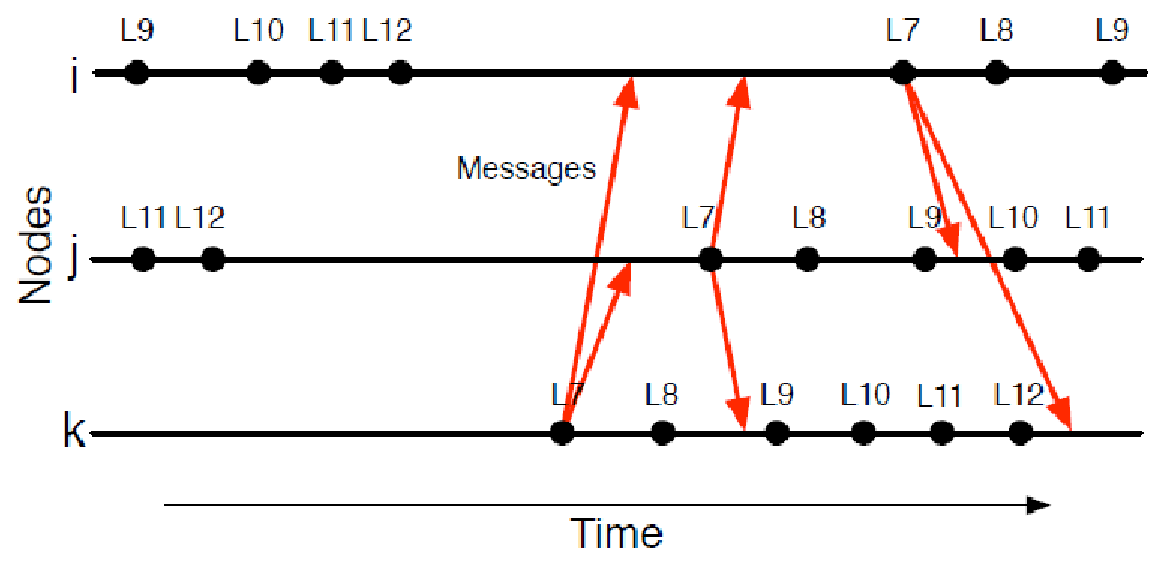
\includegraphics[scale=0.75]{fig/causality}
  \caption[Asynchronous code execution]{Nodes $i$, $j$, and $k$ execute lines of
  the macroprogram in Figure~\ref{code:ota} asynchronously.  Dots indicate when
  a node executed a particular line of code, and arrows indicate the
  transmission of cache update messages.}
  \label{fig:causallyRelated}
\end{figure}

The program in Figure~\ref{code:ota} does not include any data synchronization,
and so all nodes will execute it \emph{asynchronously}, reading from their
sensors, broadcasting their values, and calculating their own leadership status
independently of the other nodes.  Figure~\ref{fig:causallyRelated} illustrates
this asynchronous execution using a space-time diagram of three neighboring
nodes $i$, $j$, and $k$.  Time progresses from left to right and the dots on the
lines indicate the points in time when each node executes a particular line in
the macroprogram. For instance, the leftmost point on each line indicates that
the three nodes are executing lines 9, 11, and 7 of the macroprogram.  When the
nodes reach line 7 to read and store their magnetometer values, these values
automatically get reflected to neighboring nodes via a radio broadcast message
and populate the caches of the {\tt neighborMag} vector.  This is illustrated by
the arrows in the diagram.  In this example, no node is elected the leader, and
so no messages are sent to the base station when the nodes reach line 12.

% LocalWords:  macroprogram MacroLab Matlab ccc TinyDB SQL indices lightHistory
% LocalWords:  lastIndex Macrovectors DSCD microprograms RTS CAMERAFOCUS RWE ie
% LocalWords:   RWD LWARR getID getTime getProperty getNeighbors RPC extendable
% LocalWords:  getNodes distributedOperation nodeIDs funcName macrovector rts
% LocalWords:  multicast motetype groupName busstops busstop telos TinyOS JVM
% LocalWords:  online macrovectors Matlab's macroprogramming MacroLab's multi
% LocalWords:  circularBuffer lightReflection DISPAY RWED Pn CLR Whitehouse rpc
% LocalWords:  Polastre dotnetcpu sentilla embeddedPython octaveCPPCompiler
